\chapter{디랙 바다, 페르미온 질량, 그리고 4성분 스피너}

\section{오른쪽으로 움직이는 페르미온과 디랙 바다}

디랙 방정식은 페르미온을 기술하는 방정식이다. 상대론적 보손은 클라인--고든 방정식이나 맥스웰 방정식처럼 다른 방정식을 따른다. 가장 간단한 예는 공간 차원이 1인 경우로, 처음에는 오른쪽으로만 움직일 수 있는 입자와 반입자를 기술한다.

평면파에서 시작하자.
\begin{equation}
\psi(x,t)=\psi_0 e^{i(kx-\omega t)}.
\end{equation}
위상 속도는 다음과 같다.
\begin{equation}
v_{\mathrm{ph}}=\frac{\omega}{k}.
\end{equation}
\(k\)와 \(\omega\)의 부호가 중요하다. 두 부호가 같으면 위상은 오른쪽으로 움직이고, 서로 다르면 왼쪽으로 움직인다. \(\omega\)가 \(k\)에 비례하면 위상 속도와 군속도가 일치한다.
\begin{equation}
v_{\mathrm{g}}=\frac{d\omega}{dk}=\frac{\omega}{k}.
\end{equation}

다음 1계 방정식을 생각하자.
\begin{equation}
\frac{\partial\psi}{\partial x}
+
\frac{\partial\psi}{\partial t}
=0.
\end{equation}
평면파를 대입하면
\begin{equation}
ik\psi-i\omega\psi=0,
\end{equation}
이므로
\begin{equation}
\omega=k.
\end{equation}
따라서 파동은 오른쪽으로 움직인다. 이에 맞게 장에 다음과 같은 첨자를 붙이면 편리하다.
\begin{equation}
\frac{\partial\psi_R}{\partial t}
=
-\frac{\partial\psi_R}{\partial x}.
\end{equation}

빛의 속도를 다시 포함하면 차원을 갖춘 식은
\begin{equation}
\frac{\partial\psi_R}{\partial x}
+
\frac{1}{c}\frac{\partial\psi_R}{\partial t}
=0,
\end{equation}
가 되고, 따라서
\begin{equation}
\omega=ck.
\end{equation}
이제부터는 \(c=1\)로 둔다. \(\hbar=1\)이면 \(\omega\)는 양자 하나의 에너지이기도 하다.

\begin{figure}[htbp]
\centering
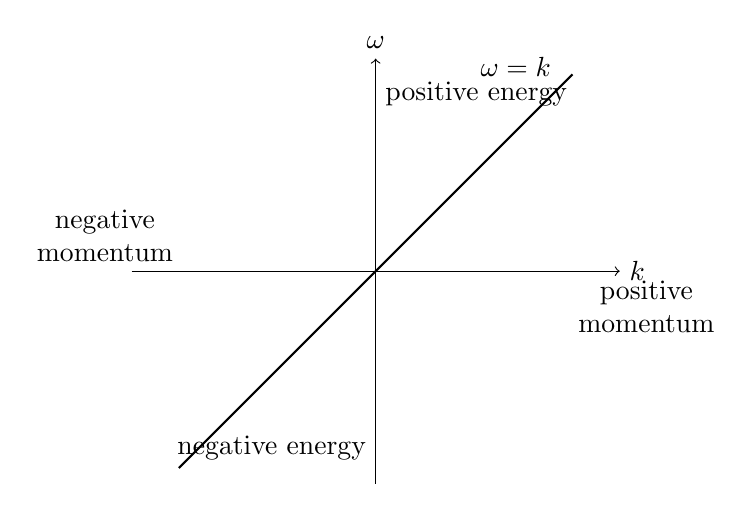
\begin{tikzpicture}[scale=1.0]
\draw[->] (-3.1,0) -- (3.1,0) node[right] {$k$};
\draw[->] (0,-2.7) -- (0,2.7) node[above] {$\omega$};
\draw[thick] (-2.5,-2.5) -- (2.5,2.5);
\node[above left] at (2.35,2.35) {$\omega=k$};
\node[below right,align=center] at (2.45,0) {positive\\momentum};
\node[above left,align=center] at (-2.45,0) {negative\\momentum};
\node[right] at (0,2.25) {positive energy};
\node[left] at (0,-2.25) {negative energy};
\end{tikzpicture}
\caption{질량이 없는 오른쪽 이동 분산 관계 \(\omega=k\)에는 양의 에너지 가지와 음의 에너지 가지가 모두 있다.}
\end{figure}

이 직선은 심각한 결과를 낳는다. \(k\)가 양수이면 에너지도 양수지만, \(k\)가 음수이면 에너지도 음수다. 그런데 직선 전체에서 \(\omega/k=1\)이므로 두 부분 모두 오른쪽으로 움직이는 파동을 나타낸다.

양의 에너지 부분에 놓인 전자는 더 낮은 상태로 떨어지며 양의 에너지를 가진 광자를 방출하고, 다시 떨어질 수 있다. 스펙트럼을 따라 한 계단, 또 한 계단, 계속 내려가는 것이다. 어떤 전자도 안정할 수 없게 된다. 더 심각하게는 음의 에너지를 가진 전자를 계속 더 많이 만들어 내면서 세계의 에너지가 낮아질 것이다.

페르미온의 배타 원리가 해결책을 제공한다. 음의 에너지를 가진 전자 상태를 모두 채우면 된다. 이미 점유된 상태에는 전자를 더 넣을 수 없으므로, 음의 에너지 영역을 완전히 채우면 무한히 떨어지는 일을 막을 수 있다. 이렇게 채워진 영역이 디랙 바다이며, 완전히 채워진 상태가 바닥 상태, 즉 진공이다.

\begin{classroomqa}
\lecturetimestamp{00:07:19}
\audiencequestion{음의 에너지 상태는 아래쪽으로 무한히 많이 있는가?}
\lecturerresponse{그렇다. 운동량이 이산적이면 스펙트럼은 무한한 계단과 같고, 연속적이면 연속적인 미끄럼틀과 같다. 음의 에너지 바다를 채우면 전자가 끝없이 내려가는 것을 막을 수 있다. 다만 점유되지 않은 더 낮은 상태가 있을 때는 광자를 방출하며 유한한 만큼 내려가는 전이가 여전히 가능하다.}
\end{classroomqa}

이 스펙트럼을 가진 방정식을 페르미온 이론으로 양자화해야 하는 이유가 여기에 있다. 양자가 보손이라면 아래쪽의 같은 상태에 얼마든지 많이 들어갈 수 있으므로, 음의 에너지 영역을 채워도 진공은 안정해지지 않는다.

바다를 채운 그림은 반입자도 설명한다. 진공에서는 모든 음의 에너지 준위가 점유되어 있고 모든 양의 에너지 준위가 비어 있다. 전자는 점유된 음의 에너지 준위 가운데 어디서든 비점유 양의 에너지 준위로 들뜰 수 있다. 처음과 나중의 준위가 서로 대칭적으로 놓여 있을 필요는 없다.

\begin{figure}[htbp]
\centering
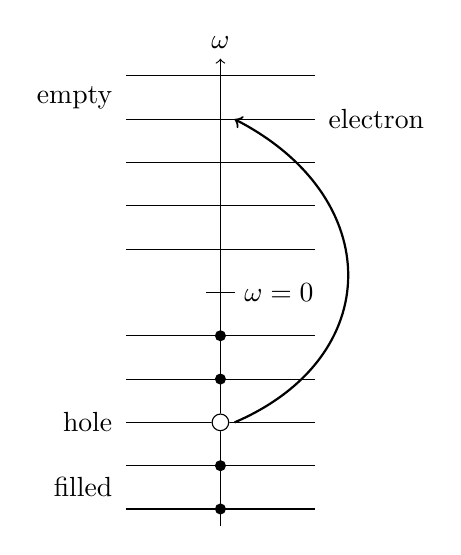
\begin{tikzpicture}[x=1cm,y=0.55cm]
\draw[->] (0,-5.4) -- (0,5.4) node[above] {$\omega$};
\draw (-0.18,0) -- (0.18,0) node[right] {$\omega=0$};
\foreach \y in {-5,-4,-3,-2,-1} {
  \draw (-1.2,\y) -- (1.2,\y);
  \fill (0,\y) circle (2pt);
}
\foreach \y in {1,2,3,4,5} {
  \draw (-1.2,\y) -- (1.2,\y);
}
\draw[->,thick] (0.18,-3) .. controls (2.1,-1.5) and (2.1,2.2) .. (0.18,4);
\draw[white,fill=white] (0,-3) circle (3pt);
\draw (0,-3) circle (3pt);
\node[left] at (-1.25,-3) {hole};
\node[left] at (-1.25,-4.5) {filled};
\node[left] at (-1.25,4.5) {empty};
\node[right] at (1.25,4) {electron};
\end{tikzpicture}
\caption{점유된 음의 에너지 전자를 들뜨게 하면 양의 에너지 전자가 생기고, 채워진 바다에는 구멍이 남는다.}
\end{figure}

음의 에너지를 가진 전자를 제거하면 진공에 비해 에너지가 올라가므로, 구멍은 양의 에너지를 갖는다. \(\omega=k\) 가지에서 제거된 전자의 운동량도 음수였다. 음의 운동량을 제거하면 양의 운동량이 남으므로, 구멍의 운동량은 양수다. 전자의 전하를 음수로 두면 전자가 빠진 자리는 양전하를 띤다. 따라서 구멍은 양의 에너지와 양의 운동량을 가진 반입자이며, 들뜬 전자는 음의 전하와 양의 에너지, 양의 운동량을 갖는다. 이 한 가지 이론의 모든 실제 들뜸은 오른쪽으로 움직인다.

장 \(\psi_R\)는 페르미온 생성 연산자와 소멸 연산자로 이루어진다. 따라서 입자와 구멍이라는 해석은 고전파만이 아니라 장이 만들고 제거하는 양자에 관한 설명이다.

여전히 비대칭성이 남아 있다. 오른쪽 이동 바다에는 음의 운동량을 가진 음의 에너지 상태가 들어 있다. 이 상태들의 형식적인 총운동량은 매우 크며 왼쪽을 향한다. 이 상수를 빼서 진공 운동량을 0으로 정의할 수는 있지만, 상태 자체의 구조적 불균형은 남는다. 입자와 반입자는 오른쪽으로만 움직이는 반면, 채워진 진공은 음의 운동량 상태로 이루어진다.

\section{왼쪽 이동 가지와 균형 잡힌 진공}

좌우 균형을 이루려면 독립적인 장 하나를 더 도입하고, 그 장에 고유한 생성 연산자와 소멸 연산자를 두어야 한다. 이 장은 다음 방정식을 따른다고 하자.
\begin{equation}
\frac{\partial\psi_L}{\partial t}
=
+\frac{\partial\psi_L}{\partial x}.
\end{equation}
같은 형태의 평면파에 대해서는
\begin{equation}
-i\omega\psi_L=ik\psi_L,
\end{equation}
이므로
\begin{equation}
\omega=-k.
\end{equation}
이 두 번째 직선은 \(\omega=k\)의 거울상이다. 양의 에너지 가지는 왼쪽으로 움직이는 입자를 나타내며, 음의 에너지 가지도 채워야 한다.

\begin{figure}[htbp]
\centering
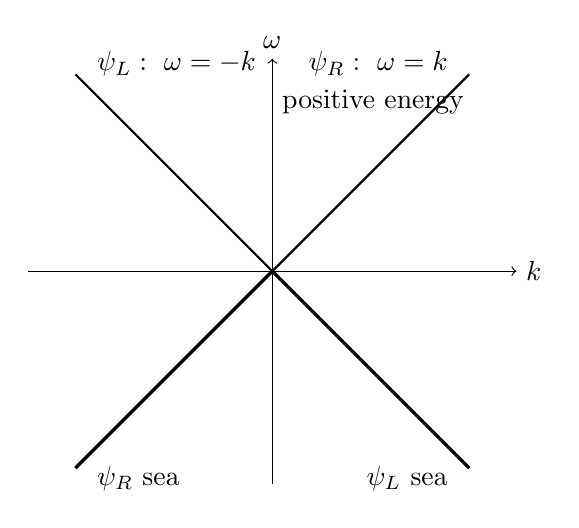
\begin{tikzpicture}[scale=1.0]
\draw[->] (-3.1,0) -- (3.1,0) node[right] {$k$};
\draw[->] (0,-2.7) -- (0,2.7) node[above] {$\omega$};
\draw[thick] (-2.5,-2.5) -- (2.5,2.5);
\draw[thick] (-2.5,2.5) -- (2.5,-2.5);
\draw[very thick] (-2.5,-2.5) -- (0,0);
\draw[very thick] (0,0) -- (2.5,-2.5);
\node[above left] at (2.35,2.35) {$\psi_R:\ \omega=k$};
\node[above right] at (-2.35,2.35) {$\psi_L:\ \omega=-k$};
\node[right] at (0,2.15) {positive energy};
\node[below right] at (-2.35,-2.35) {$\psi_R$ sea};
\node[below left] at (2.35,-2.35) {$\psi_L$ sea};
\end{tikzpicture}
\caption{독립적인 오른쪽 이동 장과 왼쪽 이동 장은 서로 거울상인 질량 없는 가지를 이루며, 두 음의 에너지 반가지가 진공에서 채워진다.}
\end{figure}

두 음의 에너지 바다를 모두 채우고 나면 점유된 왼쪽 이동 상태와 오른쪽 이동 상태의 수가 같아진다. 두 종류의 진공 운동량은 서로 상쇄된다. 이제 입자와 구멍 들뜸은 어느 쪽으로든 움직일 수 있다.

\begin{classroomqa}
\lecturetimestamp{00:15:58}
\audiencequestion{채워진 상태와 구멍을 가정하지 않고 음의 에너지 문제를 다룰 수 있는가?}
\lecturerresponse{같은 이론을 다른 방식으로 이름 붙일 수 있다. 음의 에너지 전자가 채워진 상태를 비어 있는 반입자 상태라고 부르면, 물리적 설명에는 양의 에너지를 가진 입자와 반입자만 남는다. 그래도 채워진 바다 그림은 유용한 일관성 점검 도구다. 전자를 제거하면 구멍이 생기고 들뜨게 하면 입자와 구멍이 함께 생기는 금속의 채워진 띠와 비슷하다.}
\end{classroomqa}

지금까지 다룬 들뜸은 질량이 없다. 분산 관계는 선형이고 속력의 크기는 \(1\)이므로 빛의 속도로 움직인다. 다음 질문은 이들에 질량을 어떻게 부여하느냐이다.

\section{두 성분과 질량항}

먼저 두 장을 열벡터 하나로 묶자.
\begin{equation}
\Psi=
\begin{pmatrix}
\psi_R\\
\psi_L
\end{pmatrix}.
\end{equation}
처음에는 서로 독립적인 두 방정식을 간결하게 표기한 것뿐이다. 다음을 정의하면
\begin{equation}
\alpha=
\begin{pmatrix}
1&0\\
0&-1
\end{pmatrix}.
\end{equation}
오른쪽 이동 방정식과 왼쪽 이동 방정식은 다음과 같이 된다.
\begin{equation}
\frac{\partial\Psi}{\partial t}
=
-\alpha\frac{\partial\Psi}{\partial x}.
\end{equation}

\begin{figure}[htbp]
\centering
\includegraphics[width=0.78\textwidth]{lecture_06_figure_02.png}
\caption{장 \(\psi_R\)와 \(\psi_L\)는 두 성분 스피너를 이루며, \(\alpha\)는 질량이 없는 두 가지를 구분한다.}
\lectureframe{00:20:36}
\end{figure}

평면파에 작용하는 연산자
\begin{equation}
i\partial_t
\quad\hbox{and}\quad
-i\partial_x
\end{equation}
의 값은 각각 \(\omega\)와 \(k\)이다. 따라서 행렬 방정식을 간단히 쓰면
\begin{equation}
\omega=\alpha k.
\end{equation}
위 성분에 대해서는 \(\omega=k\)을 뜻하고, 아래 성분에 대해서는 \(\omega=-k\)를 뜻한다. 이 표기는 두 방정식을 압축해 썼을 뿐 새로운 물리를 도입하지는 않는다.

전자는 질량이 없지 않으며 빛의 속도로 움직이지도 않는다. 전자의 에너지를 비상대론적 운동에너지 \(k^2/(2m)\)로 나타내고 싶을 수 있지만, 여기서 출발점으로 삼을 수는 없다. 질량이 없는 극한부터 이미 빛의 속도 운동을 다루기 때문이다. 상대론적 관계는 다음과 같다.
\begin{equation}
\omega^2=k^2+m^2,
\end{equation}
에너지의 두 가지를 모두 포함하면
\begin{equation}
\omega=\pm\sqrt{k^2+m^2}.
\end{equation}
\(m=0\)일 때 이 식들은 각각 \(\omega=k\)과 \(\omega=-k\)로 환원된다.

\begin{classroomqa}
\lecturetimestamp{00:25:23}
\audiencequestion{단위계에서 \(c=1\)로 두는가? 질량을 가진 입자의 속도는 어떻게 구하는가?}
\lecturerresponse{그렇다. 파동 묶음의 속도는 양의 에너지 가지에서 \(v_{\mathrm g}=d\omega/dk=k/\sqrt{k^2+m^2}\)인 군속도다. 따라서 질량을 가진 입자의 속력이 \(c=1\)보다 작아지는 현상이 분산 관계 자체에 담겨 있다.}
\end{classroomqa}

\begin{classroomqa}
\lecturetimestamp{00:26:29}
\audiencequestion{간략 표기 \(\omega=\alpha k\)에서 \(\omega\)는 벡터인가, 행렬인가?}
\lecturerresponse{이 간략 표기는 두 성분 파동함수에 작용하는 연산자 방정식을 뜻한다. 여기서 \(\omega\)은 \(i\partial_t\)을, \(k\)은 \(-i\partial_x\)를 뜻하며, \(\alpha\)은 성분 첨자에 작용하는 행렬이다. 스칼라 기호 \(\omega\)과 \(k\)는 평면파에서만 수치 고윳값이 된다.}
\end{classroomqa}

방정식의 차수를 1계로 유지하면서 질량에 의존하는 가장 간단한 확장을 시도하자.
\begin{equation}
\omega=\alpha k+\beta m.
\end{equation}
같은 두 성분 장에 작용하는 \(\beta\)는 행렬이어야 한다. \(\alpha\)도 그 장에 작용하기 때문이다. 제곱하면 다음과 같이 대수 관계를 얻는다.
\begin{align}
\omega^2
&=(\alpha k+\beta m)(\alpha k+\beta m)\\
&=\alpha^2k^2+\beta^2m^2
+\alpha\beta\,km+\beta\alpha\,mk\\
&=\alpha^2k^2+\beta^2m^2
+(\alpha\beta+\beta\alpha)km.
\end{align}
모든 \(k\)와 \(m\)에 대해 \(k^2+m^2\)를 얻으려면 다음을 요구해야 한다.
\begin{equation}
\alpha^2=I,
\qquad
\beta^2=I,
\qquad
\alpha\beta+\beta\alpha=0.
\end{equation}

마지막 조건은 0이 아닌 보통 수 두 개로는 만족할 수 없다. 수에 대해서는 이 조건이 \(2\alpha\beta=0\)을 뜻하는데, 두 수의 제곱이 모두 \(1\)이므로 성립하지 않는다. 행렬은 반교환할 수 있다. 특히 \(\beta\)는 \(\alpha\)와 같을 수 없다. 같다면
\begin{equation}
\alpha\beta+\beta\alpha=2\alpha^2=2I.
\end{equation}

다음과 같이 택하자.
\begin{equation}
\beta=
\begin{pmatrix}
0&1\\
1&0
\end{pmatrix}.
\end{equation}
각 성분을 계산하면 제곱을 확인할 수 있다.
\begin{equation}
\begin{aligned}
\beta^2
&=
\begin{pmatrix}
0&1\\
1&0
\end{pmatrix}
\begin{pmatrix}
0&1\\
1&0
\end{pmatrix}\\
&=
\begin{pmatrix}
0\cdot0+1\cdot1&0\cdot1+1\cdot0\\
1\cdot0+0\cdot1&1\cdot1+0\cdot0
\end{pmatrix}
=
\begin{pmatrix}
1&0\\
0&1
\end{pmatrix}.
\end{aligned}
\end{equation}
곱셈의 순서는 중요하다.
\begin{align}
\alpha\beta
&=
\begin{pmatrix}
1&0\\
0&-1
\end{pmatrix}
\begin{pmatrix}
0&1\\
1&0
\end{pmatrix}
=
\begin{pmatrix}
0&1\\
-1&0
\end{pmatrix},\\
\beta\alpha
&=
\begin{pmatrix}
0&1\\
1&0
\end{pmatrix}
\begin{pmatrix}
1&0\\
0&-1
\end{pmatrix}
=
\begin{pmatrix}
0&-1\\
1&0
\end{pmatrix}.
\end{align}
따라서
\begin{equation}
\alpha\beta=-\beta\alpha,
\qquad
\alpha\beta+\beta\alpha=0.
\end{equation}
동등한 다른 행렬을 택할 수도 있지만, 이 선택을 쓰면 성분 방정식이 특히 명확해진다.

미분 연산자를 다시 포함하면 질량이 있는 방정식은
\begin{equation}
i\frac{\partial\Psi}{\partial t}
=
-i\alpha\frac{\partial\Psi}{\partial x}
+m\beta\Psi.
\end{equation}
행렬 \(\beta\)는 두 성분을 맞바꾼다.
\begin{equation}
\beta
\begin{pmatrix}
\psi_R\\
\psi_L
\end{pmatrix}
=
\begin{pmatrix}
\psi_L\\
\psi_R
\end{pmatrix}.
\end{equation}
따라서
\begin{align}
i\dot{\psi}_R
&=-i\frac{\partial\psi_R}{\partial x}+m\psi_L,\\
i\dot{\psi}_L
&=+i\frac{\partial\psi_L}{\partial x}+m\psi_R.
\end{align}

질량항은 질량이 없는 이론에서는 서로 독립이던 장들을 결합한다. 위 성분의 방정식에는 아래 성분이 들어가고, 아래 성분의 방정식에는 위 성분이 들어간다. 이 결합이 디랙 질량의 의미다. 방정식은 병진 대칭이므로 운동량을 보존하며, 이 방정식의 입자 들뜸이 갖는 질량은 \(m\)이다.

\begin{classroomqa}
\lecturetimestamp{00:38:25}
\audiencequestion{해는 자동으로 로런츠 불변인가?}
\lecturerresponse{특정 해가 로런츠 변환 아래에서도 그대로 유지되어서는 안 된다. 운동량이 하나인 상태는 변환된 운동량을 가진 상태로 바뀌므로, 여기서 적절한 표현은 공변성이다. 관계식 \(\omega^2=k^2+m^2\)는 로런츠 불변성을 확인하는 핵심 조건 가운데 하나지만, 완전한 공변성을 보이려면 아직 정해지지 않은 스피너 \(\Psi\)의 변환 법칙도 필요하다.}
\end{classroomqa}

\section{정지계와 성분의 의미}

질량이 없는 입자는 정지 상태로 만들 수 없지만, 질량이 있는 입자는 가능하다. 정지 상태에서는 \(k=0\)이므로 파동함수는 공간적으로 변하지 않으며
\begin{equation}
\omega=\beta m.
\end{equation}
미분 방정식은 다음과 같이 줄어든다.
\begin{equation}
i\frac{d\Psi}{dt}=m\beta\Psi.
\end{equation}
성분별로 쓰면
\begin{align}
i\dot{\psi}_R&=m\psi_L,\\
i\dot{\psi}_L&=m\psi_R.
\end{align}
\(\beta\)의 비대각 성분은 둘 다 \(+1\)이므로 이 두 방정식 어느 쪽에도 별도의 마이너스 부호는 없다.

두 성분을 더하고 빼면 방정식이 분리된다. 다음과 같이 정의하자.
\begin{equation}
\psi_+=\psi_R+\psi_L,
\qquad
\psi_-=\psi_R-\psi_L.
\end{equation}
정지계 방정식 두 개를 더하면
\begin{equation}
i\dot{\psi}_+=m\psi_+,
\end{equation}
빼면
\begin{equation}
i\dot{\psi}_-=-m\psi_-.
\end{equation}
이므로
\begin{equation}
\omega=+m
\quad\hbox{for }\psi_+,
\qquad
\omega=-m
\quad\hbox{for }\psi_-.
\end{equation}

\begin{figure}[htbp]
\centering
\includegraphics[width=0.62\textwidth]{lecture_06_figure_03.png}
\caption{운동량이 0일 때 \(\psi_+=\psi_R+\psi_L\)과 \(\psi_-=\psi_R-\psi_L\)의 정지 진동수는 각각 \(\omega=+m\)과 \(\omega=-m\)이다.}
\lectureframe{00:44:49}
\end{figure}

양의 에너지 정지 장은 \(\psi_+\)이고, 음의 에너지 정지 장은 \(\psi_-\)이다. 이전과 마찬가지로 음의 에너지 상태를 채운다. 정지계 결과는 전체 스펙트럼 가운데 \(k=0\)인 단면일 뿐이다.
\begin{equation}
\omega_\pm(k)=\pm\sqrt{k^2+m^2}.
\end{equation}
\begin{figure}[htbp]
\centering
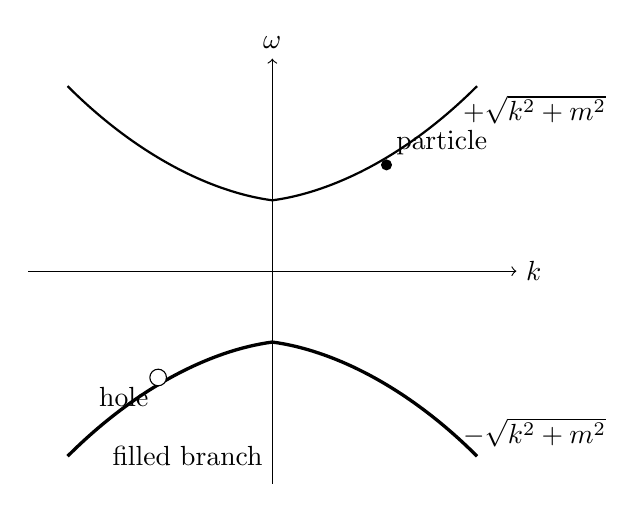
\begin{tikzpicture}[scale=1.0]
\draw[->] (-3.1,0) -- (3.1,0) node[right] {$k$};
\draw[->] (0,-2.7) -- (0,2.7) node[above] {$\omega$};
\draw[thick] (-2.6,2.35)
  .. controls (-1.7,1.45) and (-0.75,1.0) .. (0,0.9)
  .. controls (0.75,1.0) and (1.7,1.45) .. (2.6,2.35);
\draw[very thick] (-2.6,-2.35)
  .. controls (-1.7,-1.45) and (-0.75,-1.0) .. (0,-0.9)
  .. controls (0.75,-1.0) and (1.7,-1.45) .. (2.6,-2.35);
\fill (1.45,1.35) circle (2pt);
\node[above right] at (1.45,1.35) {particle};
\fill[white] (-1.45,-1.35) circle (3pt);
\draw (-1.45,-1.35) circle (3pt);
\node[below left] at (-1.45,-1.35) {hole};
\node[right] at (2.3,2.05) {$+\sqrt{k^2+m^2}$};
\node[right] at (2.3,-2.05) {$-\sqrt{k^2+m^2}$};
\node[left] at (0,-2.35) {filled branch};
\end{tikzpicture}
\caption{질량이 있는 스펙트럼에는 모든 운동량에서 양의 에너지 상태와 음의 에너지 상태가 있다. 음의 에너지 가지는 채워지며, 그 가지에서 빠진 상태는 양의 에너지를 가진 구멍이다.}
\end{figure}
모든 운동량에는 양의 에너지 상태와 음의 에너지 상태가 하나씩 있다. 음의 에너지 가지의 모든 상태를 채우면 바다 위에는 양의 에너지 입자가, 바다 안에는 양의 에너지 구멍이 남는다. 입자와 구멍 모두 질량이 양수다.

핵심을 거듭 강조할 필요가 있다. 페르미온은 원래 독립적이던 두 성분이 결합될 때 질량을 갖게 된다. 정지계에서는 원래의 어느 한 성분도 단독으로 에너지 고유상태가 아니다. 에너지가 정해진 상태는 두 성분의 합과 차이다.

합이 무엇을 뜻하는지 보려면 관련된 1입자 생성 항을 \(C_R^\dagger\)과 \(C_L^\dagger\)로 쓰자. 이를 진공에 작용시키면
\begin{equation}
(C_R^\dagger+C_L^\dagger)\lvert0\rangle
\end{equation}
두 성분이 결맞은 중첩 상태인 입자 하나가 만들어진다. 입자 두 개가 만들어지는 것은 아니다. 곱은
\begin{equation}
C_R^\dagger C_L^\dagger\lvert0\rangle,
\end{equation}
생성 연산자 두 개를 포함하므로 두 모드가 모두 가능할 때 2입자 상태를 만든다. 정규화한 정지 상태에서는 두 성분에 놓일 확률이 같지만, 결합된 파동 전체의 운동량은 0이다.

\(R\)와 \(L\)라는 명칭은 \(m=0\)일 때만 실제 운동 방향을 가리켰다. 질량항이 있으면 움직이는 질량 있는 해에는 일반적으로 두 성분이 모두 들어가며, 정지 해에도 두 성분이 같은 크기로 들어간다. 그러므로 여기서는 \(R\)와 \(L\)를 위 스피너 성분과 아래 스피너 성분의 명칭으로 보는 편이 낫다.

\begin{figure}[htbp]
\centering
\includegraphics[width=0.78\textwidth]{lecture_06_figure_04.png}
\caption{질량이 영이 아니면 두 스피너 성분은 서로 결합된다. 이 성분들을 오른쪽과 왼쪽으로 진행하는 성분으로 해석할 수 있는 것은 질량이 없는 극한에서뿐이다.}
\lectureframe{00:50:48}
\end{figure}

입자물리학의 모든 질량 있는 페르미온은 왼쪽 성분 장과 오른쪽 성분 장으로 이루어진다. 디랙 질량은 질량이 없는 극한에서 서로 독립인 성분들을 결합한다.

\begin{classroomqa}
\lecturetimestamp{00:52:01}
\audiencequestion{\(\psi_R\pm\psi_L\)에 \(1/\sqrt{2}\)를 곱해야 하는가?}
\lecturerresponse{상태를 정규화하려면 곱할 수 있다. 이 인자는 방정식의 양변에 곱해지므로 운동 방정식은 바뀌지 않는다.}
\end{classroomqa}

\begin{classroomqa}
\lecturetimestamp{00:52:12}
\audiencequestion{오른쪽 성분과 왼쪽 성분의 크기 비가 중요한가?}
\lecturerresponse{선택한 정지계 고유상태에서는 두 성분의 크기가 같다. 전체 정규화는 임의로 정할 수 있지만, 상대적인 크기는 \(\beta\)의 고유벡터가 정한다.}
\end{classroomqa}

\begin{classroomqa}
\lecturetimestamp{00:52:52}
\audiencequestion{두 성분 사이에 상대 위상이 있을 수 있는가?}
\lecturerresponse{그렇다. \(\psi_R\pm\psi_L\)에 실수 계수가 나타나는 것은 \(\beta\)를 실수로 택했기 때문이다. 단위행렬의 제곱과 같고 \(\alpha\)와 반교환하는 다른 행렬도 동등한 선택이며, 그런 경우에는 두 성분 사이에 위상이 생길 수 있다. 한 표현을 선택하면 일관되게 사용해야 한다.}
\end{classroomqa}

\begin{classroomqa}
\lecturetimestamp{00:53:43}
\audiencequestion{질량을 도입한 뒤에도 ``왼쪽 진행 성분''과 ``오른쪽 진행 성분''이라는 명칭을 써도 되나요?}
\lecturerresponse{어느 정도는 오해를 부를 수 있습니다. 질량이 없는 이론에서는 실제로 왼쪽과 오른쪽으로 진행하는 파동을 가리킵니다. 질량이 영이 아니면 한 방향으로 움직이는 입자에도 일반적으로 두 성분이 모두 들어 있으므로, ``위쪽 성분''과 ``아래쪽 성분''이라는 명칭이 더 안전합니다.}
\end{classroomqa}

\begin{classroomqa}
\lecturetimestamp{00:55:01}
\audiencequestion{정지 상태의 페르미온도 이미 스핀 각운동량을 가져야 하는가?}
\lecturerresponse{이 1차원 모형에서는 그렇지 않다. 공간 차원이 1이면 각운동량이 정의되지 않으므로 스핀은 아직 구성에 들어오지 않았다.}
\end{classroomqa}

\begin{classroomqa}
\lecturetimestamp{00:55:24}
\audiencequestion{파동함수에 페르미온 생성 연산자와 소멸 연산자가 들어 있는가?}
\lecturerresponse{그렇다.}
\end{classroomqa}

\begin{classroomqa}
\lecturetimestamp{00:55:30}
\audiencequestion{생성 연산자와 소멸 연산자를 택하는 것 말고 페르미온의 성질은 어디에서 나타나는가?}
\lecturerresponse{페르미온 생성--소멸 규칙에서 나타난다. 이러한 음의 에너지 스펙트럼을 가진 방정식은 그 규칙에 따라 양자화해야 한다. 보손의 점유 규칙을 쓰면 진공은 불안정한 채로 남는다. 상대론적 보손은 다른 파동 방정식으로 기술해야 한다.}
\end{classroomqa}

\begin{classroomqa}
\lecturetimestamp{00:56:20}
\audiencequestion{운동량이 영이 아닌 해를 로런츠 변환하여 정지계의 해로 바꿀 수 있나요?}
\lecturerresponse{네. 로런츠 부스트를 적용하면 질량이 있는 해를 정지계로 옮길 수 있습니다. 다만 그 변환을 실제로 수행하려면 로런츠 변환이 스피너 \(\Psi\)에 어떻게 작용하는지 알아야 합니다.}
\end{classroomqa}

\section{스칼라 진공장의 질량 생성}

\begin{classroomqa}
\lecturetimestamp{00:58:11}
\audiencequestion{힉스 장과의 상호작용은 어떻게 디랙 질량항을 만들어 내나요?}
\lecturerresponse{상수 질량 계수를 스칼라 장과의 결합으로 바꾸면 됩니다. 그 장이 진공에서 영이면 페르미온은 질량이 없는 상태로 남고, 일정한 영이 아닌 진공값을 가지면 그 결합은 질량과 정확히 같은 역할을 합니다.}
\end{classroomqa}

\(\phi(x,t)\)를 자체 운동 방정식이 있는 스칼라장이라고 하자. 디랙 방정식의 질량항에서 상수 \(m\)를 \(g\phi(x,t)\)로 바꾼다.
\footnote{\(m\beta\Psi\)에 표시된 상호작용항은 앞서 정한 질량항에 이 치환을 적용해 얻는다.}
\begin{equation}
i\frac{\partial\Psi}{\partial t}
=
-i\alpha\frac{\partial\Psi}{\partial x}
+g\phi(x,t)\,\beta\Psi.
\end{equation}
그러면 두 장의 방정식이 서로 결합된다. 페르미온은 스칼라장에 작용하고 스칼라장은 다시 페르미온에 작용한다. 디랙 방정식은 주어진 \(\phi\)에 대해 \(\Psi\)에 선형이지만, 두 장을 함께 보면 계 전체는 비선형이다.

먼저 빈 공간에 다음과 같은 장이 있다고 하자.
\begin{equation}
\phi(x,t)=0.
\end{equation}
그러면 혼합항이 사라지고 위쪽 성분과 아래쪽 성분이 분리되어 페르미온은 질량이 없다. 반대로 가장 낮은 에너지 상태에서 스칼라 장이 일정한 영이 아닌 값을 가진다고 하자.
\begin{equation}
\phi(x,t)=\phi_0\neq0.
\end{equation}
그 진공에서 디랙 방정식은 다음과 같이 된다.
\begin{equation}
i\frac{\partial\Psi}{\partial t}
=
-i\alpha\frac{\partial\Psi}{\partial x}
+g\phi_0\,\beta\Psi,
\end{equation}
따라서
\begin{equation}
m_{\mathrm{eff}}=g\phi_0.
\end{equation}
이처럼 보손 장과 페르미온 장의 결합에 더해 빈 공간에서 보손 장이 영이 아닌 값을 가지면, 이전에는 방정식에 질량으로 직접 넣었던 것과 같은 좌우 성분 간 혼합이 생긴다.

\begin{classroomqa}
\lecturetimestamp{01:01:27}
\audiencequestion{LHC가 진공에서 힉스 장이 영이 아님을 보여 주는 증거를 제공할 수 있을까요?}
\lecturerresponse{물론입니다. 그것은 중요한 쟁점 중 하나입니다.}
\end{classroomqa}

\begin{classroomqa}
\lecturetimestamp{01:01:32}
\audiencequestion{힉스 메커니즘이 어떻게 작동하는지 좀 더 설명해 주실 수 있나요?}
\lecturerresponse{스칼라 장은 공간과 시간에 따라 변할 때 에너지를 가지며, 국소 퍼텐셜 에너지 \(V(\phi)\)도 가질 수 있습니다. 퍼텐셜의 최솟값이 \(\phi\)의 영이 아닌 값에서 나타난다면 진공에는 영이 아닌 장이 존재합니다. 선택된 최솟값 주위에서 양자화된 진동이 힉스 입자입니다.}
\end{classroomqa}

장은 서로 구별되는 두 방식으로 에너지를 가질 수 있다. 일부 에너지는 장이 공간과 시간에 따라 어떻게 변하는지에 달려 있다. 익숙한 비교 대상으로 맥스웰 장을 들 수 있다.
\begin{equation}
\mathcal{E}_{\mathrm{Maxwell}}\propto \mathbf E^2+\mathbf B^2,
\end{equation}
\(\mathbf E\)과 \(\mathbf B\)는 모두 전자기 퍼텐셜의 미분으로 이루어진다. 따라서 이 에너지는 바탕이 되는 장의 시공간 변화와 관련된다.

스칼라장은 국소 퍼텐셜 에너지 밀도도 가질 수 있다.
\begin{equation}
V(\phi),
\end{equation}
이는 미분값이 아니라 \(\phi\) 자체의 값에 달려 있다. 개략적으로 쓰면
\begin{equation}
\mathcal{E}_\phi
=
\mathcal E_{\text{space and time gradients}}+V(\phi).
\end{equation}
더 깊은 원리가 값을 정해 주지 않는 한, \(V(\phi)\)는 모형의 대칭과 양립하는 임의의 그럴듯한 함수일 수 있다.

여기서 사용하는 단순화된 실수 스칼라 예에서는 이론이 다음 변환에 대해 대칭이라고 하자.
\begin{equation}
\phi\longrightarrow-\phi.
\end{equation}
그러면 퍼텐셜은 짝함수여야 한다.
\begin{equation}
V(\phi)=V(-\phi).
\end{equation}
이 대칭만으로는 최솟값이 어디에 있는지 알 수 없다. 한 가지 가능성은 \(\phi=0\)에 최솟값 하나가 있는 것이다. 또 다른 가능성은 영이 아닌 값에서 대칭적인 두 최솟값, 즉 양의 값과 음의 값 하나씩이 나타나는 것이다.

\begin{figure}[htbp]
\centering
\includegraphics[width=0.72\textwidth]{lecture_06_figure_05.png}
\caption{최솟값이 \(\phi=0\)에 있으면 진공 장은 영이 된다. 반면 대칭적인 영이 아닌 최솟값에서는 진공값 \(\phi_0\neq0\)이 허용되고, 따라서 페르미온 질량 \(g\phi_0\)도 생긴다.}
\lectureframe{01:04:47}
\end{figure}

퍼텐셜의 구체적인 다항식 형태를 정하지 않고도 두 가능성을 그림으로 나타낼 수 있다.\footnote{아래 곡선에는 논의에 필요한 중앙의 최솟값과 대칭으로 짝을 이루는 최솟값만 질적으로 나타냈다.}
\begin{figure}[htbp]
\centering
\resizebox{\linewidth}{!}{%
\begin{tikzpicture}[x=1.35cm,y=1.05cm]
\begin{scope}[shift={(-3.1,0)}]
\draw[->] (-1.7,0) -- (1.7,0) node[right] {$\phi$};
\draw[->] (0,-0.15) -- (0,2.45) node[above] {$V(\phi)$};
\draw[thick] (-1.5,2.05) .. controls (-0.9,0.65) and (-0.45,0.25) .. (0,0.25)
             .. controls (0.45,0.25) and (0.9,0.65) .. (1.5,2.05);
\fill (0,0.25) circle (1.2pt);
\node[below] at (0,0) {$0$};
\end{scope}
\begin{scope}[shift={(3.1,0)}]
\draw[->] (-1.7,0) -- (1.7,0) node[right] {$\phi$};
\draw[->] (0,-0.15) -- (0,2.45) node[above] {$V(\phi)$};
\draw[thick] (-1.55,2.05)
  .. controls (-1.25,0.75) and (-1.0,0.25) .. (-0.75,0.25)
  .. controls (-0.35,0.25) and (-0.25,1.3) .. (0,1.3)
  .. controls (0.25,1.3) and (0.35,0.25) .. (0.75,0.25)
  .. controls (1.0,0.25) and (1.25,0.75) .. (1.55,2.05);
\fill (-0.75,0.25) circle (1.2pt);
\fill (0.75,0.25) circle (1.2pt);
\node[below] at (0,0) {$0$};
\node[below] at (-0.75,0) {$-\phi_0$};
\node[below] at (0.75,0) {$\phi_0$};
\end{scope}
\end{tikzpicture}%
}
짝함수 퍼텐셜에는 중앙의 최솟값 하나가 있을 수도 있고, 대칭을 이루는 영이 아닌 최솟값 두 개가 있을 수도 있다.\caption{
}
\end{figure}

최솟값이 원점에 있으면 진공은 \(\phi_0=0\)이고, 이 결합은 전자에 질량을 주지 않는다. 최솟값이 \(\phi=\pm\phi_0\)에 있으면 진공은 둘 중 하나에 자리 잡는다. 두 선택은 대칭으로 연결되어 있으며, 어느 쪽을 택해도 디랙 방정식에 영이 아닌 계수 \(g\phi_0\)가 생긴다. 퍼텐셜이 왜 이런 질적 형태를 갖는지는 더 깊은 문제이며, 이 메커니즘 자체로 답할 수는 없다.

장은 반드시 최솟값에만 머물 필요는 없다. 입자가 퍼텐셜 우물 바닥 근처에서 진동하듯 선택된 값 주위에서 진동할 수 있다. 이 진동을 양자화하면 힉스 양자가 생긴다. 그 특성 진동수는 힉스 입자 질량과 관련된다. 질량이 크면 양자 하나를 들뜨게 하는 데도 많은 에너지가 필요하다. 진공에서는 장이 최솟값 부근에 머물면서 페르미온 질량을 제공한다. 장이 진동하면 그 진동이 힉스 입자다.

이 결합에는 작용과 반작용이 따른다. 페르미온은 \(\phi\)의 값에 반응하지만, 충분히 에너지가 큰 페르미온 충돌은 스칼라장도 들뜨게 할 수 있다. 충돌은 들뜸에 필요한 에너지를 공급해야 한다. 장이 진동하면 그 양자가 힉스 입자다. 이 장은 전자뿐 아니라 쿼크장과 질량을 부여하는 다른 장에도 결합한다.

\begin{classroomqa}
\lecturetimestamp{01:08:14}
\audiencequestion{힉스장이 진동하거나 변위하면 전자 질량도 변하는가?}
\lecturerresponse{그렇다. 유효 질량은 장의 국소적인 값에 비례하므로 장을 0 쪽으로 변위시키면 질량이 작아진다. 거시적인 영역을 진공값에서 멀리 떨어진 상태로 유지하려면 막대한 에너지가 필요하다. 그런 실험을 할 수 있을 만큼 큰 영역은 블랙홀로 붕괴할 수도 있다.}
\end{classroomqa}

사고실험은 간단하다. 한 영역을 \(\phi=0\) 부근에 붙들어 둘 수 있다면, 그 영역 안에서는
\begin{equation}
m_{\mathrm{eff}}=g\phi
\end{equation}
가 작아지거나 사라질 것이다. 들뜬 힉스 모드는 진공값 주위에서 진동하지만, 거시적 영역 전체에 걸쳐 상당한 변위를 만들고 유지하려면 막대한 에너지가 든다. 퍼텐셜 에너지 비용은 부피에 따라 커진다. 그런 영역이 실용적인 실험실이 되기 훨씬 전에 에너지가 중력 붕괴를 일으킬 만큼 커질 수 있다. 원리적으로 질량 변화는 실제지만, 관측 가능한 큰 변화를 일으키기는 극도로 어렵다.

\begin{classroomqa}
\lecturetimestamp{01:09:27}
\audiencequestion{힉스장이 필요한 이유는 무엇인가?}
\lecturerresponse{전자에 질량이 있기 때문이다.}
\end{classroomqa}

\begin{classroomqa}
\lecturetimestamp{01:09:41}
\audiencequestion{입자 종류마다 고유한 힉스장이 있는가?}
\lecturerresponse{아니다. 표준모형에서는 하나의 힉스장이 전자, 쿼크 및 이 메커니즘에 참여하는 다른 입자에 질량을 부여한다. 초대칭 이론에서는 입자 종류마다 별도의 장을 두는 대신 힉스장이 두 개 필요하다.}
\end{classroomqa}

하나의 장으로 설명하는 그림은 개략적이다. 실제 힉스장은 실수 하나 \(\phi\)보다 더 복잡한 구조를 갖는다. 그래도 핵심은 그대로다. 하나의 공통 진공장이 페르미온마다 서로 다른 세기로 결합할 수 있으므로, 입자 종류마다 서로 다른 힉스장을 둘 필요는 없다. 힉스 입자는 그 동일한 장이 진공값 주위에서 진동하는 것이다.

힉스장을 도입하지 않고 전자 질량을 방정식에 그냥 넣으면 되지 않을까? 그 답은 약한 상호작용과 통일에 관련되어 있으며, 여기서는 뒤로 미룬다.

\begin{classroomqa}
\lecturetimestamp{01:11:16}
\audiencequestion{초대칭 이론에는 힉스 부문이 두 개 있는가?}
\lecturerresponse{그렇다. 여기서 사용하는 단순화된 구분에 따르면 하나는 업형 쿼크에 질량을 주고, 다른 하나는 다운형 쿼크와 전자에 질량을 준다. 힉스장이 두 배 필요한 것은 초대칭의 기술적 요구이지, 입자마다 별도의 힉스장을 두기 때문은 아니다.}
\end{classroomqa}

\begin{classroomqa}
\lecturetimestamp{01:12:01}
\audiencequestion{힉스 입자에 질량이 있다면 그 질량은 어디서 오는가?}
\lecturerresponse{이 질문은 여기서 해결하지 않는다. 더 정확히 말하면, 힉스 질량이 왜 그렇게 작은지가 수수께끼다.}
\end{classroomqa}

대칭성은 질량 문제와 분리될 수 없다. 단순한 디랙 모형에서는 왼쪽 부문과 오른쪽 부문이 서로 섞이지 않도록 하는 대칭성 때문에 혼합항의 계수가 영이어야 한다. 진공이 그 대칭성을 따랐다면 페르미온은 질량이 없었을 것이다. 영이 아닌 힉스 진공값은 관련된 진공 대칭성을 깨뜨려 좌우 결합을 허용한다:
\begin{equation}
m_{\mathrm{eff}}=g\phi_0\neq0.
\end{equation}
정확한 대칭 변환은 여기서 전개하지 않는다. 여기서 중요한 점은 그것이 질량항에 미치는 결과다. 특정한 최저 에너지 상태가 대칭성을 따르지 않더라도 방정식 자체는 대칭성을 가질 수 있다. 질량을 부여하는 것은 바로 진공의 이러한 비대칭성이다.

여기서 개괄하는 전약 이론에서는 전자와 쿼크뿐 아니라 \(W\) 보손과 \(Z\) 보손도 이 방식으로 질량을 얻는다. 광자는 질량이 없다. 힉스 입자 자체는 또 다른 예외다. 같은 진공 변위가 없어도 질량을 가질 수 있으며, 그 질량은 좌우 페르미온 성분의 혼합이 아니라 힉스 장 자체의 진동과 관련된다. 따라서 이 설명에서 힉스 진공값은 다른 입자들의 질량을 만들지만, 힉스 들뜸의 질량은 별도의 질문을 제기한다.

\begin{classroomqa}
\lecturetimestamp{01:15:26}
\audiencequestion{중력자는 질량이 있나요?}
\lecturerresponse{아니요. 중력자는 광자처럼 질량이 없습니다. 중성미자도 한때 질량이 없다고 여겨졌지만, 실제로는 매우 작은 질량을 가집니다. 여기서 설명한 언어로 말하면, 이는 중성미자의 왼쪽 성분과 오른쪽 성분의 결합이 매우 약하다는 뜻입니다.}
\end{classroomqa}

광자와 이론상 중력자는 질량이 없으며 빛의 속도로 움직인다. 중성미자는 이 부류에 완전히 속하지 않는다. 중성미자의 극히 작은 질량은 디랙 이론에서 두 성분을 결합하는 항이 극히 작다는 뜻이다. 왜 그 값이 그렇게 작은지는 또 다른 문제다.

\section{3차원 공간에서의 디랙 방정식}

3차원 공간에서는 파수가 파수 벡터가 된다.
\begin{equation}
\mathbf{k}=(k_1,k_2,k_3),
\end{equation}
이 벡터는 \(x\), \(y\), \(z\) 방향의 성분을 갖는다. 1차원 관계식에는 다음 부호가 들어간다.
\begin{equation}
\omega=\alpha k+\beta m,
\end{equation}
이를 가장 단순하게 선형 일반화하면 다음과 같다.
\begin{equation}
\omega
=
\alpha_1 k_1+\alpha_2 k_2+\alpha_3 k_3+\beta m.
\end{equation}
여기서 \(\alpha_i\)와 \(\beta\)는 행렬이다. 이 행렬들은 다음 조건을 만족하도록 정해야 한다.
\begin{equation}
\omega^2=k_1^2+k_2^2+k_3^2+m^2.
\end{equation}
이 불변 분산 관계는 필수 조건이지만, 이것만으로 상대성 이론의 내용을 모두 담지는 못한다.

선형식을 제곱하면 다음과 같다.
\begin{align}
\omega^2
={}&
\alpha_1^2k_1^2+\alpha_2^2k_2^2+\alpha_3^2k_3^2+\beta^2m^2
\nonumber\\
&+(\alpha_1\alpha_2+\alpha_2\alpha_1)k_1k_2
+(\alpha_1\alpha_3+\alpha_3\alpha_1)k_1k_3
\nonumber\\
&+(\alpha_2\alpha_3+\alpha_3\alpha_2)k_2k_3
+\sum_{i=1}^{3}(\alpha_i\beta+\beta\alpha_i)k_i m.
\end{align}
운동량 제곱항과 질량항의 계수는 다음 조건을 요구한다.
\begin{equation}
\alpha_1^2=\alpha_2^2=\alpha_3^2=I,
\qquad
\beta^2=I.
\end{equation}
원치 않는 \(k_i k_j\) 항은 서로 다른 \(\alpha\) 행렬들이 반교환하면 사라진다.
\begin{equation}
\alpha_i\alpha_j+\alpha_j\alpha_i=0,
\qquad i\neq j.
\end{equation}
혼합된 \(k_i m\) 항은 다음 조건에서 사라진다.
\begin{equation}
\alpha_i\beta+\beta\alpha_i=0
\qquad
\text{for each }i.
\end{equation}
따라서 네 행렬은 모두 항등행렬을 제곱으로 가지며, 서로 다른 행렬은 어느 두 개를 택해도 반교환한다.

서로 반교환해야 하는 조건을 만족하는 \(2\times2\) 행렬 세 개는 실제로 존재한다. 이들은 세 파울리 행렬이다. 항등행렬을 제곱으로 가지면서 세 행렬 모두와 반교환하는 네 번째 \(2\times2\) 행렬은 없다. \(3\times3\) 행렬을 사용하는 표현도 불가능하다. 가능한 가장 작은 표현은 \(4\times4\) 행렬을 사용하는 디랙 행렬 표현이다.

성분 수를 두 개에서 네 개로 늘리면 물리적 의미에 관한 질문이 생긴다. 한 차원 공간에서 두 성분은 왼쪽과 오른쪽으로 진행하는 장으로 시작했다. 네 성분은 무엇을 뜻할까? 새롭게 들어오는 것은 스핀이다. 스핀을 다루려면 각운동량이 필요하므로, 공간이 실제로 3차원인 경우를 논의해야 한다.

행렬의 표현은 하나로 정해져 있지 않다. 서로 직교하는 좌표축을 여러 방식으로 선택해도 동등한 것과 마찬가지로, 여러 선택은 서로 동등하다. 행렬의 성분은 달라지지만 변환을 통해 서로 다른 기술을 연결할 수 있고 물리는 변하지 않는다. 편리한 한 표현은\footnote{아래의 성분별 행렬은 바로 뒤에 제시된 블록 형식과 파울리 행렬을 전개한 것이다. 이 블록 관계는 강의에서 명시적으로 서술되어 있다013023--013129}
\begin{equation}
\beta=
\begin{pmatrix}
1&0&0&0\\
0&1&0&0\\
0&0&-1&0\\
0&0&0&-1
\end{pmatrix},
\end{equation}
그리고
\begin{align}
\alpha_1&=
\begin{pmatrix}
0&0&0&1\\
0&0&1&0\\
0&1&0&0\\
1&0&0&0
\end{pmatrix},
&
\alpha_2&=
\begin{pmatrix}
0&0&0&-i\\
0&0&i&0\\
0&-i&0&0\\
i&0&0&0
\end{pmatrix},
\\[1ex]
\alpha_3&=
\begin{pmatrix}
0&0&1&0\\
0&0&0&-1\\
1&0&0&0\\
0&-1&0&0
\end{pmatrix}.
\end{align}
각 행렬을 \(2\times2\) 블록으로 나누면 그 구조를 더 쉽게 파악할 수 있다:
\begin{equation}
\beta=
\begin{pmatrix}
I_2&0\\
0&-I_2
\end{pmatrix},
\qquad
\alpha_i=
\begin{pmatrix}
0&\sigma_i\\
\sigma_i&0
\end{pmatrix}.
\end{equation}
세 파울리 행렬은 다음과 같다:
\begin{equation}
\sigma_1=
\begin{pmatrix}
0&1\\
1&0
\end{pmatrix},
\quad
\sigma_2=
\begin{pmatrix}
0&-i\\
i&0
\end{pmatrix},
\quad
\sigma_3=
\begin{pmatrix}
1&0\\
0&-1
\end{pmatrix}.
\end{equation}
이 블록 행렬들은 필요한 디랙 반교환 관계를 만족한다.

이제 파동함수는 네 성분을 가져야 한다.
\begin{equation}
\Psi=
\begin{pmatrix}
\psi_1\\
\psi_2\\
\psi_3\\
\psi_4
\end{pmatrix}.
\end{equation}
운동 방정식은 다음과 같다.
\begin{equation}
i\frac{\partial\Psi}{\partial t}
=
-i\sum_{j=1}^{3}\alpha_j
\frac{\partial\Psi}{\partial x_j}
+\beta m\Psi.
\end{equation}
이 간결한 식은 서로 결합된 네 개의 선형 미분방정식을 나타낸다. \(\alpha_j\)의 비대각 원소는 1차원 경우보다 더 복잡한 방식으로 네 성분을 서로 결합하지만, 기본 구조는 같다. 행렬이 성분들을 결합하는 한편 방정식은 공간과 시간에 대해 여전히 1계 미분방정식이다. 성분 수가 다시 두 배로 늘어난 점이 스핀으로 이어지는 단서다.

\begin{classroomqa}
\lecturetimestamp{01:33:53}
\audiencequestion{\(\Psi\)의 네 성분은 시공간의 네 차원에 직접 대응하는 4-벡터인가요?}
\lecturerresponse{아니요. 이들은 4-벡터가 아니라 스피너를 이룬다. 1차원 공간의 예에서 시공간 차원 수와 스피너 성분 수가 둘로 같았던 것은 우연이다. 고차원 구성에서 스피너 행렬의 크기는 2의 거듭제곱으로 나타나며, 일반적으로 시공간 차원 수와 같지 않다.}
\end{classroomqa}

정지계에서 다시 가장 간단한 해석을 얻는다. 운동량이 0이면 미분항이 사라진다.
\begin{equation}
i\frac{\partial\Psi}{\partial t}=m\beta\Psi.
\end{equation}
선택한 표현에서 \(\beta\)의 고윳값은 \(+1\) 두 개와 \(-1\) 두 개다. 따라서 에너지 \(+m\)인 정지 상태가 두 개, 에너지 \(-m\)인 정지 상태도 두 개다. 앞서와 마찬가지로 음의 에너지 상태들은 채워진다. 에너지 부호마다 두 겹으로 중복되는 이 구조가 스핀의 물리적 해석에 필요한 추가 구조다.

\begin{classroomqa}
\lecturetimestamp{01:35:51}
\audiencequestion{\(\alpha_i\)의 비대각 블록은 같은 아래첨자를 달아 \(\sigma_i\)로 해야 하나요?}
\lecturerresponse{네. 각 행렬 \(\alpha_i\)에는 해당 파울리 행렬 \(\sigma_i\)이 두 비대각 블록에 모두 들어갑니다.}
\end{classroomqa}

\begin{classroomqa}
\lecturetimestamp{01:36:03}
\audiencequestion{\(\alpha_i\)의 간결한 반교환 관계식에는 계수 2가 빠져 있나요?}
\lecturerresponse{네. \(i=j\)이면 좌변은 \(\alpha_i^2+\alpha_i^2=2I\)입니다. 올바른 관계식은 \(\alpha_i\alpha_j+\alpha_j\alpha_i=2\delta_{ij}I\)입니다.}
\end{classroomqa}

따라서 제곱 조건과 서로 다른 첨자에 대한 조건을 하나로 합치면 다음과 같다.
\begin{equation}
\alpha_i\alpha_j+\alpha_j\alpha_i=2\delta_{ij}I.
\end{equation}

\begin{classroomqa}
\lecturetimestamp{01:36:42}
\audiencequestion{디랙이 구성 과정에서 행렬을 네 개로 늘린 것은 개념적으로 큰 도약이었나요?}
\lecturerresponse{네. 디랙은 방정식을 가정하고 그 결과를 추적했습니다. 그 결과 중 하나는 반입자의 출현이었고, 또 하나는 스핀이었다. 스핀은 이미 실험적으로 알려져 있었지만, 이 방정식은 스핀을 설명했다.}
\end{classroomqa}

\begin{classroomqa}
\lecturetimestamp{01:37:29}
\audiencequestion{입자가 보손과 페르미온으로 제한된다는 정리와 실험적 증거 중 무엇이 먼저 나왔나요?}
\lecturerresponse{실험적 증거가 먼저였고 정리는 나중에 나왔습니다. 보손--페르미온의 양자택일은 공간이 3차원일 때 적용됩니다. 시간 차원이 하나인 2차원 공간에서는 중간 통계가 나타날 수 있지만, \(3+1\)차원 이상의 공간에서는 보손과 페르미온만 가능합니다.}
\end{classroomqa}

\begin{classroomqa}
\lecturetimestamp{01:39:01}
\audiencequestion{\(\Psi\)의 네 성분에 통상적으로 쓰는 첨자가 있습니까?}
\lecturerresponse{여기서는 반드시 택해야 하는 첨자가 정해져 있지 않습니다. \(p\)와 \(q\)를 첨자로 쓸 수 있으며, 각각 1부터 4까지의 값을 가집니다. 그러면 각 행렬은 행 첨자 하나와 열 첨자 하나를 가집니다.}
\end{classroomqa}

행렬 표기에서는 이 성분 첨자들이 생략된다. 첨자를 명시하면 다음과 같다.
\begin{equation}
p,q=1,2,3,4,
\end{equation}
그러면 방정식은 다음과 같이 쓸 수 있다.
\begin{equation}
i\,\partial_t\Psi_p
=
-i\sum_{j=1}^{3}\sum_{q=1}^{4}
(\alpha_j)_{pq}\,\partial_j\Psi_q
+m\sum_{q=1}^{4}\beta_{pq}\Psi_q.
\end{equation}

\begin{classroomqa}
\lecturetimestamp{01:40:15}
\audiencequestion{행렬 곱을 사용하면 성분 첨자를 굳이 쓰지 않아도 되나요?}
\lecturerresponse{네. 행렬 표기에서는 그러한 첨자가 자동으로 생략됩니다. 상대론적 구조를 더 분명하게 드러내는 대칭적인 형태는 나중에 도입할 수 있습니다.}
\end{classroomqa}

제시된 방정식은 가장 단순한 \(3+1\)차원 형태의 디랙 방정식이다. 다음 단계에서는 스핀을 이해하고 상대론적 보손의 파동 방정식을 세워야 한다. 디랙 방정식은 보손을 기술하는 방정식이 아니며, 자연계 입자의 약 절반은 보손이기 때문이다. 이런 요소들을 갖추면 쿼크, 렙톤, 약한 보손, 힉스 입자와 광자를 살펴보고 입자 스펙트럼을 어느 정도 체계화할 수 있다. 이 논의 전반에는 더 많은 대칭이 필요하다.
